\documentclass[10pt]{article}

\pagestyle{empty}

\setlength{\textheight}{250mm}
\setlength{\textwidth}{180mm}
\setlength{\oddsidemargin}{-8mm}
\setlength{\topmargin}{-1.5cm}

\usepackage{amsmath}
\usepackage{amsthm}
\usepackage{psfrag}
\usepackage{graphicx}
\usepackage{bm}
\usepackage{mathrsfs}
\usepackage{icomma} % pacchetto per limitare lo spazio standard posto dopo la virgola in caso che la virgola sia tra cifre
\usepackage{amsfonts} % amplia i caratteri matematici disponibili
\usepackage{amssymb}
%\usepackage{wrapfig}
\usepackage{empheq}

\usepackage{epstopdf}
\usepackage[utf8x]{inputenc}
\usepackage{ifthen}
\usepackage{subfig}

\usepackage[italian]{babel}
%\usepackage[latin1]{inputenc}

\usepackage{pgfplots}
\pgfplotsset{compat=1.9}

%\input{def}

%\newcommand{\kg}{\textrm{kg}}
%\newcommand{\K}{\textrm{K}}
%\newcommand{\m} {\textrm{m}}
%\newcommand{\dm}{\textrm{dm}}
%\newcommand{\cm}{\textrm{cm}}
%\newcommand{\mm}{\textrm{mm}}
%\newcommand{\s} {\textrm{s}}
%\newcommand{\N} {\textrm{N}}
%\renewcommand{\Pa}{\textrm{Pa}}

\def \flagSect{0} % 1    : numerazione
		  % else : niente
%\newcommand{\taitol}[1]  % stile titolo
%{
%%{\textit{#1}}
%{#1}
%}
\def \soluzione{Soluzione}
\def \partePrima{Concetti. }
\def \parteSeconda{Svolgimento. }
%\def \parteTerza{}
\newcommand{\sol}{\subsubsection*{\soluzione}}
\newcommand{\partone}{\ \ \ \ \ \textbf{\partePrima}}
\newcommand{\parttwo}{\vspace{0.2cm}\textbf{\parteSeconda}}

\ifnum\flagSect=1
\newtheorem{esercizio}{Esercizio}%[section]
\else
\newtheorem*{esercizio}{Esercizio}
\fi

\newtheorem*{teorema}{Teorema}
\newtheorem*{lemma}{Lemma}

% ###########################################################
%\def \flagSect{0} % 1    : numerazione
		  % else : niente
%\newcommand{\taitol}[1]  % stile titolo
%{
%%{\textit{#1}}
%{#1}
%}
\def \soluzione{Soluzione}
\def \partePrima{Concetti. }
\def \parteSeconda{Svolgimento. }
%\def \parteTerza{}
\newcommand{\sol}{\subsubsection*{\soluzione}}
\newcommand{\partone}{\ \ \ \ \ \textbf{\partePrima}}
\newcommand{\parttwo}{\vspace{0.2cm}\textbf{\parteSeconda}}

\ifnum\flagSect=1
\newtheorem{esercizio}{Esercizio}%[section]
\else
\newtheorem*{esercizio}{Esercizio}
\fi

\newtheorem*{teorema}{Teorema}
\newtheorem*{lemma}{Lemma}

% ###########################################################
%\def \flagSect{0} % 1    : numerazione
		  % else : niente
%\newcommand{\taitol}[1]  % stile titolo
%{
%%{\textit{#1}}
%{#1}
%}
\def \soluzione{Soluzione}
\def \partePrima{Concetti. }
\def \parteSeconda{Svolgimento. }
%\def \parteTerza{}
\newcommand{\sol}{\subsubsection*{\soluzione}}
\newcommand{\partone}{\ \ \ \ \ \textbf{\partePrima}}
\newcommand{\parttwo}{\vspace{0.2cm}\textbf{\parteSeconda}}

\ifnum\flagSect=1
\newtheorem{esercizio}{Esercizio}%[section]
\else
\newtheorem*{esercizio}{Esercizio}
\fi

\newtheorem*{teorema}{Teorema}
\newtheorem*{lemma}{Lemma}

% ###########################################################
%\input{logicNumb}
%\newcommand{\sectionIf}[2]
%{
%   \ifthenelse{\equal{#1}{1}}
%              {\subsection{#2}}{\subsection*{#2}}
%}
% ###########################################################

%\newcommand{\sectionIf}[2]
%{
%   \ifthenelse{\equal{#1}{1}}
%              {\subsection{#2}}{\subsection*{#2}}
%}
% ###########################################################

%\newcommand{\sectionIf}[2]
%{
%   \ifthenelse{\equal{#1}{1}}
%              {\subsection{#2}}{\subsection*{#2}}
%}
% ###########################################################



\begin{document}

\begin{center}
\textbf{Esercizi per il corso di Fluidodinamica} 
\medskip
\end{center}


\begin{minipage}[l]{0.45\textwidth}
 \begin{exerciseS}[Strato limite di Blasius 3D]
  Nella figura accanto una lastra piana di corda $c=30\ cm$, apertura $b=75\ cm$ 
  e spessore trascurabile \`{e} investita da una 
  corrente esterna d'aria ($\rho=1.225\ kg/ m^3$, $\mu=1.76\times10^{-5}\ kg/(ms)$) 
  uniforme in corda e variabile in apertura secondo la legge 
\[
\bm{U}_e(z) = U_e(z) \mathbf{\hat{\bm{x}}} = \overline{U} \left( \frac{z}{b} \right)^{2/3} \mathbf{\hat{\bm{x}}}
\]
con $\overline{U}=5\ m/s$. Assumendo la corrente
  laminare, stazionaria e bidimensionale su ciascuna sezione $z$ in apertura, 
  e potendone approssimare lo strato limite attraverso la soluzione di Blasius, 
  si richiede di:
  \begin{itemize}
   \item[2.1)] calcolare la resistenza $D$ della lastra ed il corrispondente momento 
               all'incastro $M_y$;
           \item[2.2)] calcolare lo spessore di spostamento $\delta^*(x,z)$ e di quantit\`{a} 
               di moto $\theta(x,z)$ dello strato limite sulla superficie della lamina;
%              al bordo d'uscita della 
%              lamina con riferimento alla sezione di mezzeria. 
%              Calcolare il rapporto di forma $H=\delta^*/\theta$.
  \end{itemize}
%  \vspace{1cm}
%  (Si ricorda che per la soluzione di Blasius il fattore di forma $H$, definito come il rapporto $\delta^*/\theta$, risulta $H=2.59$ e che 
%   $f''(0)=0.332$.)
 \end{exerciseS}
\end{minipage}
\hspace{3mm}
\begin{minipage}[r]{0.55\textwidth}
  \centering
  \vspace{5mm}
  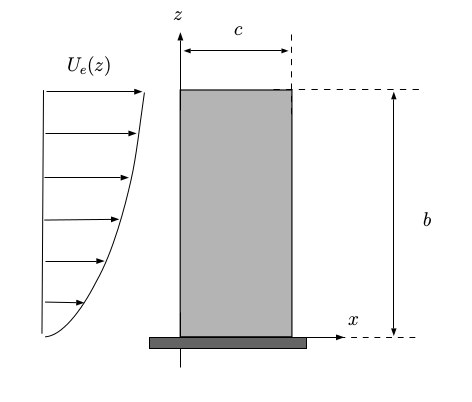
\includegraphics[width=1.0\textwidth]{./fig/sheet}
\end{minipage}

% ---------------------------------------------------------------------------

\sol

\partone Soluzione di Blasius dello strato limite. Spessori di strato limite.

\vspace{0.5cm}
\parttwo
 Assumendo valido il modello 2D di Blasius per lo strato limite \textit{quasi-3D} del problema, lo spessore convenzionale dello strato limite vale
 \begin{equation}
     \delta(x,z) = \sqrt{ \dfrac{x \nu}{ U_e(z)} } \ ,
 \end{equation}
 e lo sforzo viscoso a parete in direzione $x$ vale
 \begin{equation}
     \tau_w(x,z) = \mu \dfrac{\partial u}{\partial y}\Bigg|_{y=0} = 
     \mu \, g''(0) \dfrac{U_e(z)}{\delta(x,z)} = 
     g''(0) \mu \dfrac{U_e^{3/2}(z)}{\sqrt{\nu x}}  \ .
     = g''(0) \sqrt{ \mu \rho } \dfrac{U_e^{3/2}(z)}{\sqrt{x}}  \ .
 \end{equation}
 Utilizzando il profilo di velocità fornito dal problema,
 \begin{equation}
     \delta(x,z) = \sqrt{\dfrac{x \nu b^{1/3}}{ \overline{U} z^{1/3} }} \qquad , \qquad
     \tau_w(x,z) = g''(0) \sqrt{ \mu \rho } \, \dfrac{\overline{U}^{3/2}}{b} \dfrac{z}{\sqrt{x}}  \ .
 \end{equation}
 
 \begin{itemize}
 
 \item 
 Per il calcolo della resistenza e del momento alla radice è necessario calcolare
 lo sforzo a parete sulla lamina piana $\tau_w (x,z)$. La resistenza è l'integrale
 di $\tau_w$ sulla superficie; il momento $M_y$ è l'integrale di $z \tau_w (x,z)$
 esteso alla superficie,
 % (viene fatta l'ipotesi che l'unica componente dello sforzo a parete sia diretta lungo x).
\begin{equation}
  D = \int_{x=0}^{c} \int_{z=0}^b \tau_w(x,z) dx \, dz = 
    g''(0) \sqrt{ \mu \rho } \, \overline{U}^{3/2} \, b \, \sqrt{c} \ ,
\end{equation}
\begin{equation}
  M_y = \int_{x=0}^{c} \int_{z=0}^b z \tau_w(x,z) dx \, dz = 
    \dfrac{2}{3} g''(0) \sqrt{ \mu \rho } \, \overline{U}^{3/2} \, b^2 \, \sqrt{c} \ .
\end{equation}

 \item
  Nel modello \textit{quasi-3D} dello strato limite, gli spessori integrali sono funzione di $(x,z)$,
  \begin{equation}
   \delta^*(x,z) = \int_0^\infty \displaystyle\left[ 1 - \frac{u(x,y,z)}{U_e(x,z)} \right] dy ,\qquad
   \theta(x,z) = \int_0^\infty \frac{u(x,y,z)}{U_e(x,z)} \displaystyle\left[ 1 - \frac{u(x,y,z)}{U_e(x,z)} \right] dy \ ,  
  \end{equation}
  e utilizzando le relazioni dello strato limite di Blasius
 \begin{equation}
     \delta^*(x,z) = 1.721 \, \delta(x,z) \qquad , \qquad
       \theta(x,z) = 0.644 \, \delta(x,z) \ .
 \end{equation}

%  Usando le relazioni dello strato limite di Blasius, si trova
%  \begin{equation}
%  \begin{aligned}
%  & \delta^* = \int_0^\infty (1 - g'(\eta(y))) dy = 
%      \delta(x) \int_0^\infty (1 - g'(\eta)) d\eta \\
%  & \theta   = \int_0^\infty g'(\eta) (1 - g'(\eta(y))) dy = 
%      \delta(x) \int_0^\infty g'(\eta) (1 - g'(\eta)) d\eta
%  \end{aligned}
%  \end{equation}
%  
%  Per lo spessore di spostamento si ha:
%  \begin{equation}
%  \begin{aligned}
%   \delta^* & = \delta(x) \int_0^\infty (1 - g'(\eta)) d\eta = 
%          & \\
%            & = \delta(x) [\eta - g(\eta)]|_0^\infty = 
%          & \text{($g(0) = 0$)} \\
%            & = \delta(x) \lim_{\eta \to \infty} [\eta - g(\eta)] = 
%          & \text{($\lim_{\eta \to \infty} [\eta - g(\eta)] = 1.721$)} \\
%            & = 1.721 \cdot \delta = 
%          & \text{($\delta = \sqrt{\nu x / U}$)} \\
%            & = 1.721 \sqrt{\frac{\nu x}{U(z)}}
%  \end{aligned}
%  \end{equation}
%  
%  Per lo spessore di quantità di moto:
%  \begin{equation}
%  \begin{aligned}
%   \theta   & = \delta(x,z) \int_0^\infty g'(\eta) (1 - g'(\eta)) d\eta = & \\
%            & = \delta \int_0^\infty g'(\eta) d\eta 
%                 - \delta \int_0^\infty g'^2(\eta) d\eta = & \\
%            & = \delta [g(\eta)]|_0^\infty 
%                 - \delta \int_0^\infty g'^2(\eta) d\eta = 
%          & \text{($g(0)=0$ e IxP)} \\
%            & = \delta \lim_{\eta \to \infty}  g(\eta) 
%                 - \delta \int_0^\infty [(g g')' - g g''] d\eta = 
%          & \text{(eq. di Blasius: $\frac{1}{2}g g'' + g''' = 0$)} \\
%            & = \delta \lim_{\eta \to \infty}  g(\eta) 
%                 - \delta [g g']|_0^\infty 
%                 - \delta \int_0^\infty 2 g''' d\eta = 
%          & \text{($g(0) = 0$)}\\
%            & = \delta \lim_{\eta \to \infty}  g(\eta)
%                 - \delta \lim_{\eta \to \infty}  g(\eta)g'(\eta)
%                 - 2 \delta [g''(\eta)]|_0^\infty = 
%          & \text{($\lim_{\eta \to \infty} g'(\eta) = 1$, 
%            $\lim_{\eta \to \infty} g''(\eta) = 0$)} \\
%            & = 2 \delta(x,z) g''(0) = \\
%            & = 0.664 \sqrt{\frac{\nu x}{U(z)}}
%  \end{aligned}
%  \end{equation}
%  
%  Il rapporto di forma vale quindi $H = \delta^* / \theta = 1.721 / 0.664$, cioè
%  $H = 2.59$.
 
%  \vspace{1.0cm}
%  \begin{figure*}[h!]
%  \centering
%    \subfloat[]
%    [\emph Grafico di $g(\eta)$: per $\eta \to \infty$ g ha derivata uguale a $1$; l'intersezione dell'asintoto con l'asse orizzontale avviene per $g(0)=1.721$.]
%      {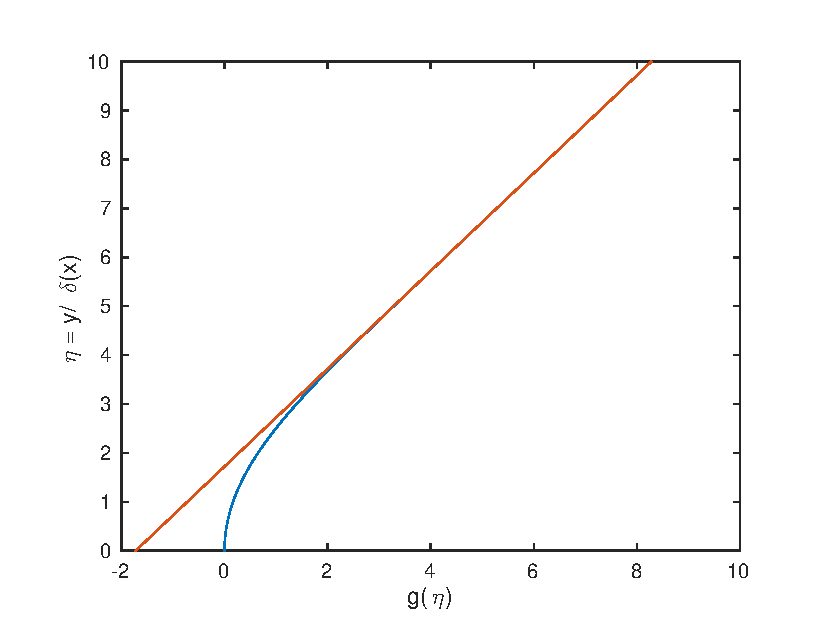
\includegraphics[width=.31\textwidth]{./fig/BlasiusShooting/g.eps}} \quad
%    \subfloat[]
%    [\emph Grafico di  $g'(\eta)$: rappresenta il profilo adimensionale dela velocità. Per
%    $\eta \to \infty$ $g'(\eta) \to 1$.]
%      {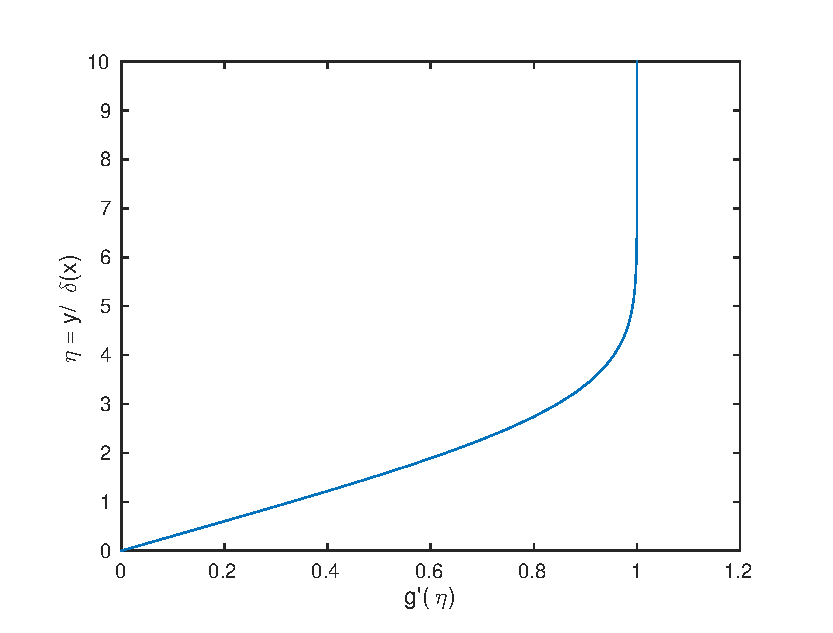
\includegraphics[width=.31\textwidth]{./fig/BlasiusShooting/dg.eps}} \quad
%    \subfloat[]
%    [\emph Grafico di $g''(\eta)$: è legato alla derivata parziale $\partial u / \partial y$. 
%    Per determinare lo sforzo a parete è necessario trovare il valore di $g''(0)$: $g''(0) = 0.332$]
%      {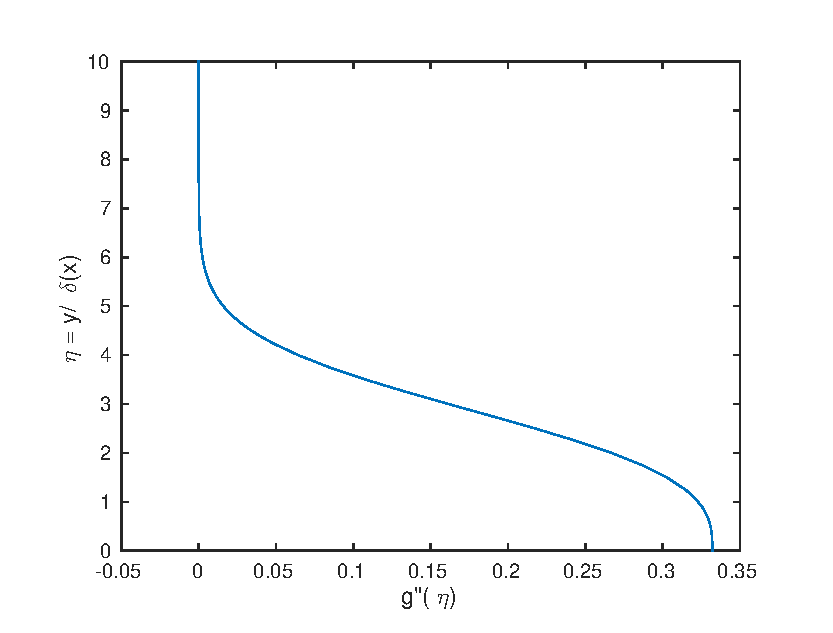
\includegraphics[width=.31\textwidth]{./fig/BlasiusShooting/ddg.eps}}
% \end{figure*}
 
 \end{itemize}









%%%%%%%%%%%%%%%%%%%%%%%%%%%%%%%%%%%%%%%%%%%%%%%%%%%%%%%%%%%%%%%%%%

%%%%%%%%%%%%%%%%%%%%%%%%%%%%%%%%%%%%%%%%%%%%%%%%%%%%%%%%%%%%%%%%%%

%%%%%%%%%%%%%%%%%%%%%%%%%%%%%%%%%%%%%%%%%%%%%%%%%%%%%%%%%%%%%%%%%%



%%%%%%%%%%%%%%%%%%%%%%%%%%%%%%%%%%%%%%%%%%%%%%%%%%%%%%%%%%%%%%%%%%

%%%%%%%%%%%%%%%%%%%%%%%%%%%%%%%%%%%%%%%%%%%%%%%%%%%%%%%%%%%%%%%%%%
%%%%%%%%%%%%%%%%%%%%%%%%%%%%%%%%%%%%%%%%%%%%%%%%%%%%%%%%%%%%%%%%%%

\end{document}
